\documentclass[12pt]{extarticle}
%Some packages I commonly use.
\usepackage[portuguese]{babel}
\usepackage{graphicx}
\usepackage{framed}
\usepackage[normalem]{ulem}
\usepackage{amsmath}
\usepackage{amsthm}
\usepackage{amssymb}
\usepackage{amsfonts}
\usepackage{enumerate}
\usepackage[utf8]{inputenc}
\usepackage{float}
\usepackage{gensymb}
\usepackage[top=1 in,bottom=1in, left=1 in, right=1 in]{geometry}
\usepackage{multirow}
\usepackage{caption}
\usepackage{subcaption}
\usepackage[utf8]{inputenc}

%A bunch of definitions that make my life easier
\newcommand{\matlab}{{\sc Matlab} }
\newcommand{\cvec}[1]{{\mathbf #1}}
\newcommand{\rvec}[1]{\vec{\mathbf #1}}
\newcommand{\ihat}{\hat{\textbf{\i}}}
\newcommand{\jhat}{\hat{\textbf{\j}}}
\newcommand{\khat}{\hat{\textbf{k}}}
\newcommand{\minor}{{\rm minor}}
\newcommand{\trace}{{\rm trace}}
\newcommand{\spn}{{\rm Span}}
\newcommand{\rem}{{\rm rem}}
\newcommand{\ran}{{\rm range}}
\newcommand{\range}{{\rm range}}
\newcommand{\mdiv}{{\rm div}}
\newcommand{\proj}{{\rm proj}}
\newcommand{\R}{\mathbb{R}}
\newcommand{\N}{\mathbb{N}}
\newcommand{\Q}{\mathbb{Q}}
\newcommand{\Z}{\mathbb{Z}}
\newcommand{\<}{\langle}
\renewcommand{\>}{\rangle}
\renewcommand{\emptyset}{\varnothing}
\newcommand{\attn}[1]{\textbf{#1}}
\theoremstyle{definition}
\newtheorem{theorem}{Theorem}
\newtheorem{corollary}{Corollary}
\newtheorem*{definition}{Definition}
\newtheorem*{example}{Example}
\newtheorem*{note}{Note}
\newtheorem{exercise}{Exercise}
\newcommand{\bproof}{\bigskip {\bf Proof. }}
\newcommand{\eproof}{\hfill\qedsymbol}
\newcommand{\Disp}{\displaystyle}
\newcommand{\qe}{\hfill\(\bigtriangledown\)}
\setlength{\columnseprule}{1 pt}
\usepackage[utf8]{inputenc}

\title{Aula 29 - Quantidade de Movimento, Colisões e Análise Dimensional}
\author{Felipe Salvador}
\date{Atualizado em \today}

\begin{document}

\maketitle

\section{Introdução}
Nesta aula, nós trataremos uma parte da física responsável por descrever o choque entre 2 corpos. Passaremos pelos diversos tipos de colisões e enunciaremos principais quantidades responsáveis pela descrição. No fim de cada parte, terá um exemplo para ilustrar como cada tipo de colisão funciona e como se chega nos resultados.

\section{Quantidade de Movimento (Momento Linear) - $Q$}

A principal quantidade física envolvida nas colisões é a chamada \textbf{Quantidade de Movimento ou Momento Linear}\footnote{Normalmente, em materiais do Ensino Médio é usado o nome Quantidade de Movimento, enquanto em materiais de Ensino Superior é chamado de Momento Linear. Não sei bem dizer o porquê da diferença de terminologia, mas coloquei no texto ambas as terminologias porque não há um consenso sobre qual usar.}. Essa quantidade é definida como:
\begin{equation}
    Q = m\,v
\end{equation}
\noindent em que $m$ é a massa do corpo e $v$ é a sua velocidade. Perceba que, se o corpo estiver parado, a quantidade de movimento será 0. E, conforme o corpo se movimenta mais rapidamente, maior será a quantidade.

Nos processos de colisões, o conceito mais importante é a \textbf{Conservação da Quantidade de Movimento} - quer dizer que, a quantidade de movimento total antes da colisão é igual à quantidade de movimento total depois da colisão. Em \textit{matematiquês}, isso é:
\begin{equation}
    (Q_{total})_i = (Q_{total})_f
\end{equation}
\noindent em que $Q_{total}$ é a soma de todas as quantidades de movimentos dos corpos envolvidos na colisão.
Caso a colisão envolva 2 corpos, a equação acima fica assim:
\begin{equation}
    Q_{1i} + Q_{2i} = Q_{1f} + Q_{2f}
\end{equation}
\noindent em que $Q_{1i}$ é a quantidade de movimento do corpo 1 antes da colisão, $Q_{2f}$ é a quantidade de movimento do corpo 2 após a colisão e assim por diante.

Como $Q=m\,v$, então:
\begin{equation}
    m_1\,v_{1i} + m_2\,v_{2_i} = m_1\,v_{1f}+m_2\,v_{2f}
\end{equation}

\begin{figure}[H]
    \centering
    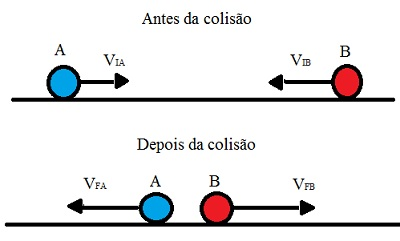
\includegraphics[width=0.6\textwidth]{colisao.jpg}
    \caption{Esquema de uma colisão de 2 corpos}
    \label{fig:colisao}
\end{figure}

\section{Colisões}
\subsection{Colisão Elástica}
\textbf{A colisão elástica é aquela que a energia cinética total das massas colidindo é conservada.} Ou seja, em relação matemática, isso é dado como:
\begin{equation}\label{eq:energy_cons}
    \begin{split}
        &(E_c)_{1i} + (E_c)_{2i} = (E_c)_{1f} + (E_c)_{2f}\\
        & \frac{m_1\,v_{1i}^2}{2} + \frac{m_2\,v_{2i}^2}{2} = \frac{m_1\,v_{1f}^2}{2} + \frac{m_2\,v_{2f}^2}{2}
    \end{split}
\end{equation}

Além da energia, o quantidade de movimento também é conservada:
\begin{equation}\label{eq:momentum_cons}
    m_1\,v_{1i} + m_2\,v_{2i} = m_1\,v_{1f} + m_2\,v_{2f}
\end{equation}

Com isso, as equações \ref{eq:energy_cons} e \ref{eq:momentum_cons} são as equações a serem resolvidas no problema. Para resolvê-las, precisamos de 4 das 6 informações do problema ($m_1,\,m_2,\,v_{1i},\,v_{2i},\,v_{1f},\,v_{2f}$). As outras 2 informações são deduzidas a partir das equações acima.

Um exemplo clássico de colisões elásticas é a colisão de 2 bolas de sinuca. Vamos usá-las no exemplo a seguir:

\textit{Exemplo 1:} Duas bolas de sinuca, a bola A com massa de 50,0 g e a bola B com massa de 40,0 g, se colidem. Antes da colisão, a bola A estava se movimentando com velocidade $v_0 = 5 m/s$, enquanto a bola B estava em repouso. O sistema é descrito pela figura abaixo. Determine as velocidades finais das bolas.

\begin{figure}[H]
    \centering
    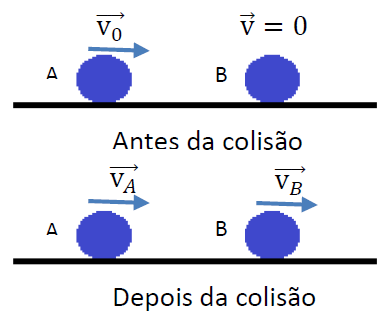
\includegraphics[width=0.4\textwidth]{elastica.png}
    \label{fig:ex_1}
\end{figure}

Para determinar as velocidades finais, temos que usar as relações de conservação. Pela Conservação de Quantidade de Movimento:
\begin{equation}\label{eq:ex_1}
    \begin{split}
        &0,05*5 + 0,04*0 = 0,05*v_{1f} + 0,04*v_{2f}\\
        &100*0,25 = 5*v_{1f} + 4*v_{2f}\\
        &5*v_{1f} + 4*v_{2f} = 25 \implies \boxed{v_{1f} = \frac{25 - 4*v_{2f}}{5}}
    \end{split}
\end{equation}

Pela Conservação de Energia, temos:
\begin{equation}
    \begin{split}
        &\frac{0,05*5^2}{2} + \frac{0,04*0^2}{2} = \frac{0,05*v_{1f}^2}{2} + \frac{0,04*v_{2f}^2}{2}\\
        &0,05*25 = 0,05*v_{1f}^2 + 0,04*v_{2f}^2\\
        &100*1,25= 5*v_{1f}^2 + 4*v_{2f}^2
    \end{split}
\end{equation}

Substituindo o resultado da equação \ref{eq:ex_1} no lugar de $v_{1f}$:
\begin{equation}
    \begin{split}
        &125= 5*\left(\frac{25 - 4*v_{2f}}{5}\right)^2 + 4*v_{2f}^2\\
        &125= \frac{25^2 - 2*25*4*\,v_{2f} + 16*v_{2f}^2}{5} + 4*v_{2f}^2\\
        & 125*5 = 25^2 - 2*25*4*\,v_{2f} + 16\,v_{2f}^2 + 5*4\,v_{2f}^2\\
        &625 = 625-200\,v_{2f} + (16+20)\,v_{2f}^2\\
        &36\,v_{2f}^2 - 200\,v_{2f} =0
    \end{split}
\end{equation}
Colocando $v_{2f}$ em evidência:
\begin{equation}
        v_{2f}\left(36\,v_{2f} - 200\right) =0
\end{equation}
Como o produto é igual à 0, então um dos fatores é 0. Ou seja:
\begin{equation}
    \begin{split}
        &v_{2f} =0\\
        &36\,v_{2f} - 200=0 \implies v_{2f} = \frac{200}{36}
    \end{split}
\end{equation}

Bem, as duas respostas estão certas? Não, pois como os objetos são bolas que tem massas bem parecidas, então é esperado que numa colisão, a segunda bola entre em movimento também. Por isso, a resposta $v_{2f}=0$ é descartada. Logo, a resposta certa é (fazendo a fatoração):
\begin{equation}
    \boxed{v_{2f} = \frac{50}{9}\, m/s = 5,55...\, m/s}
\end{equation}

Com isso, podemos retornar o valor para o resultado dado por \ref{eq:ex_1}:
\begin{equation}
    \begin{split}
            &v_{1f} = \frac{25 - 4*\frac{50}{9}}{5} = \frac{25 - \frac{200}{9}}{5} = \frac{\frac{25*9 - 200}{9}}{5} = \frac{25*9 -200}{5*9} = \frac{225-200}{45}=\frac{25}{45}\\
            &\boxed{v_{1f} = \frac{5}{9}\, m/s = 0,555...\,m/s}
    \end{split}
\end{equation}

Logo, na colisão, a bola A transfere quase que toda a velocidade para a bola B e sobra 0,555... m/s para a bola A. Isso é bem comum de acontecer na sinuca, em que a bola A é a bola branca e a bola B são as bolas a serem encaçapadas. Se a tacada não bem ajustada e sem efeito na bola branca, essa sobra de velocidade pode fazer com que a bola branca vá para a caçapa junto com a bola colorida.

\subsection{Colisão Inelástica}

\textbf{São as colisões em que os objetos se grudam após a colisão e se movem juntos com a mesma velocidade.} Nesse caso, a energia total dos objetos \textbf{não} é conservada, então: $(E_{total})_i > (E_{total}){f}$. Isso é válido, porque essa diferença de energia é usada para deformar ou alterar a estrutura interna dos objetos na colisão inelástica. Um diagrama de uma colisão inelástica está a seguir:
\begin{figure}[H]
    \centering
    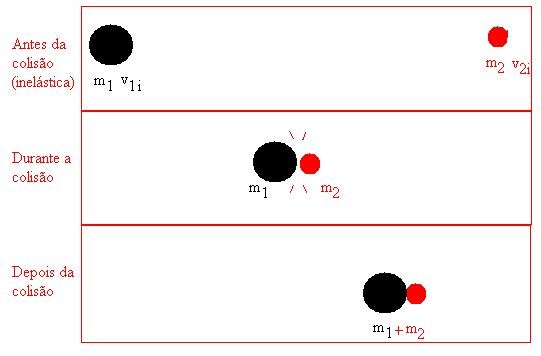
\includegraphics[width=0.6\textwidth]{inelastica.jpg}
    \caption{Diagrama de uma colisão inelástica}
    \label{fig:inelastica}
\end{figure}

Com isso, a conservação da quantidade de movimento é dada como:
\begin{equation}\label{eq:inelastic}
    m_1\,v_1 + m_2\,v_2 = m_1\,v + m_2\,v \implies \boxed{m_1\,v_1 + m_2\,v_2 = (m_1+ m_2)\,v}
\end{equation}
\noindent em que $v_1,v_2$ são as velocidades iniciais do objeto 1 e 2, respectivamente, $m_1,\,m_2$ são os valores das massas e $v$ é a velocidade após a colisão (lembrando que os dois objetos ficam grudados).

\textit{Exemplo 2:} Um bloco de massa de 1 kg se move com velocidade de 5 m/s e vá de encontro a um pêndulo cuja ponta tem uma massa de 5 kg e está em repouso. Essa massa é feita de um material colante de forma que no momento em que o bloco se chocar com a massa do pêndulo, eles grudam e ficam unidos. O sistema todo está descrito na figura abaixo.

\begin{figure}[H]
    \centering
    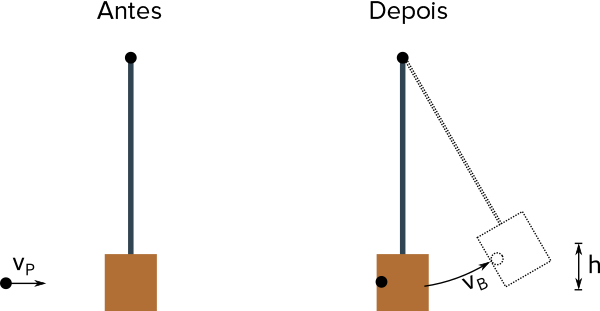
\includegraphics[width=0.5\textwidth]{example_2.png}
    \label{fig:ex_2}
\end{figure}

Encontre a velocidade do conjunto após a colisão. Qual é a altura máxima que o pêndulo irá atingir após a colisão?

Para a primeira pergunta, vamos usar a conservação da quantidade de movimento para uma colisão inelástica dada pela equação \ref{eq:inelastic}, usando os dados do problema:
\begin{equation}
    1*5 + 5*0 = (5+1)\,v \implies \boxed{v = \frac{5}{6}\, m/s \approx 0,83\, m/s}
\end{equation}

Para a segunda parte, após a colisão, o pêndulo irá subir por causa da velocidade. Para achar a altura, iremos usar a conservação de energia. Logo após a colisão, o conjunto tem a velocidade encontrada e vai subir. Na altura máxima, o pêndulo está parado momentaneamente e depois volta a descer. Então, a conservação de energia é:
\begin{equation}
    \begin{split}
        (E_c)_i + (E_p)_i = (E_c)_f + (E_p)_f
    \end{split}
\end{equation}

\noindent em que $(E_c)_i$ é a energia cinética inicial do conjunto, $(E_p)_i$ é a energia potencial gravitacional inicial e o subíndice 'f' são as energias cinética e potencial gravitacional final.

No início, a energia cinética é dada por $(E_c)_i = \frac{m\,v^2}{2} \frac{(5+1)\,(5/6)^2}{2}$ e a energia potencial gravitacional é $(E_p)_i=0$. No final, a energia cinética é: $(E_c)_f = 0$ e a energia potencial gravitacional é: $(E_p)_f = (5+1)\,10\,h$, em que $g=10\,m/s^2$. Logo, a conservação de energia é:
\begin{equation}
    \begin{split}
        &\frac{6*\left(\frac{5}{6}\right)^2}{2} = 6*10\,h\\
        &\frac{\frac{25}{6}}{2} = 20\,h\\
        &\frac{25}{12} = 20\,h \\
        &h = \frac{5}{48} \implies \boxed{h \approx 0,10\, m}
    \end{split}
\end{equation}

\section{Coeficiente de Restituição (e)}

O coeficiente de restituição é uma quantidade que me diz sobre a velocidade relativa que um corpo se afasta do outro corpo após uma colisão. Essa quantidade é definida como:
\begin{equation}
    e = \frac{|v_{1f} - v_{2f}|}{|v_{2i}-v_{1i}|}
\end{equation}

Essa quantidade é adimensional, ou seja, não tem unidade. Ela caracteriza cada tipo de colisão que existe na natureza:
\begin{table}[H]
    \centering
    \begin{tabular}{|c|c|}
    \hline
         \textbf{Tipo de Colisão} & \textbf{Valor de $e$}   \\
         \hline 
         Colisão Elástica & e=1\\
         \hline
         Colisão Parcialmente Elástica & $0<e<1$\\
         \hline
         Colisão Inelástica & e=0\\
         \hline
    \end{tabular}
    \caption{Tabela com os tipos de colisão e os valores do coeficiente de restituição}
    \label{tab:coef_restituicao}
\end{table}

As colisões parcialmente elásticas são colisões em que os corpos se colidem, mas não grudam (como nas colisões inelásticas), mas a energia total do problema \textbf{não} é conservada. Fazem parte da grande maioria das colisões na natureza.

\section{Análise Dimensional}

Análise Dimensional é uma técnica usada para descobrir, conferir ou entender qual é uma grandeza relacionada a outras grandezas conhecidas. No Sistema Internacional (SI), há 7 grandezas primárias:
\begin{itemize}
    \item \textbf{Comprimento [L] - metro (m)} 
    \item \textbf{Tempo [T] - segundo (s)}
    \item \textbf{Massa [M] - quilograma (kg)}
    \item \textbf{Intensidade da corrente elétrica [I] - Ampère (A)}
    \item \textbf{Temperatura [$\theta$] - Kelvin (K)}
    \item \textbf{Intensidade Luminosa [$I_0$] - Candela (Cd)}
    \item \textbf{Quantidade de matéria [N] - mol (mol)}
\end{itemize}

A partir delas, construímos todas as outras quantidades que vimos nas aulas por meios das equações que construímos/vimos. Um exemplo é a velocidade e a aceleração. Sabemos que a velocidade é dada por:
\begin{equation}
    v= \frac{\Delta S}{\Delta t} \implies [v] = \frac{[\Delta S]}{[\Delta t]} = \frac{[L]}{[T]} \implies \boxed{[v] = \frac{m}{s}}
\end{equation}
\noindent em que quando colocamos uma grandeza dentro de colchetes, estamos analisando a sua unidade. Vemos que a unidade da velocidade é metros por segundo, no Sistema Internacional. Agora, vamos analisar a aceleração:
\begin{equation}
    a= \frac{\Delta v}{\Delta t} \implies [a] = \frac{[\Delta v]}{[\Delta t]} = \frac{[v]}{[T]} = \frac{m/s}{s} \implies \boxed{[a] = \frac{m}{s^2}}
\end{equation}
E dessa forma, vamos construindo todas as unidades que vimos no ano. Podemos, por fórmulas diferentes, ver que 2 quantidades são uma mesma grandeza. Um exemplo é a energia cinética e a energia potencial gravitacional:
\begin{equation}
    E_c = \frac{mv^2}{2} \implies[E_c] = \frac{[m][v^2]}{[2]} = [M][V]^2 \implies \boxed{[E_c] = \frac{kg\,m^2}{s^2} = J}
\end{equation}
Mas, pela energia potencial gravitacional:
\begin{equation}
     E_p = mgh \implies[E_p] = [m][g][h] = [M][a][L] \implies \boxed{[E_c] = kg\,\frac{m}{s^2}\,m = \frac{kg\,m^2}{s^2} = J}
\end{equation}
Olha só, é a mesma unidade!!! Além disso, sempre que vemos uma quantidade com unidade $\frac{kg\,m^2}{s^2}$ já sabemos que se trata de energia, pois essa unidade é a definição da unidade Joule.

Por que a Análise Dimensional é tão importante para uma prova? Porque caso você esqueça da fórmula, mas lembre da unidade da grandeza e como essa unidade é escrita, você consegue deduzir a fórmula para essa grandeza (a menos de constante adimensionais, que não tem como descobrir nesse método).

Mas, pelo menos, esse método é um grande salva-vidas numa prova, quando a pressão, estresse são altos e a chance de dar branco numa fórmula é razoável. Por isso que treinar Análise Dimensional é uma excelente arma para esses casos numa prova!!!

\end{document}
